All measurements take place at room temperature.
\subsection{Set up}
\begin{figure}[htbp]
	\centering
		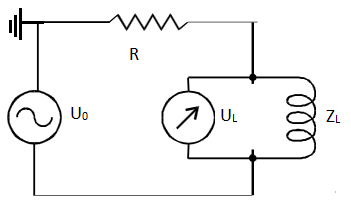
\includegraphics[width=0.50\textwidth]{img/circuit}
	\caption{schematic of the electric circuit used in the experiment\cite{coilImpedance}}
	\label{fig:circuit}
\end{figure}

\begin{figure}[htbp]
	\centering
		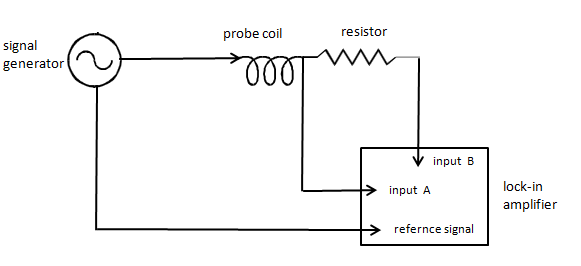
\includegraphics[width=0.50\textwidth]{img/setup}
	\caption{schematic of the set up of the electric equipment}
	\label{fig:setup}
\end{figure}
First, we built a probe coil with impedance $Z_L$ by spooling a copper wire on a ferrite core. Then, we connected this coil together with a resistor $R=1\text{ k}\Omega$ to a signal generator that provides a complex voltage $V_0=0.1\text{ V}\cdot\text{e}^{2\pi\text{j}f}$ as shown in schematic \ref{fig:circuit}, and \ref{fig:setup}. A 2-input lock-in voltmeter is used to measure the voltage over the resistor as well as the voltage over probe and resistor combined. This allows us to measure the voltage $U_L$ over the probe, too, since the voltmeter can calculate the difference between its two input signals. The probe coil can be moved manually to scan sample surfaces. 

\subsection{Crack Detection}
For the crack detection test, we put the coil on the surface of a sample in such a way that the coil's magnetic field enters the sample perpendicular to the surface. We measured the coil voltage $U_L$ at different positions of the probe relative to a visible crack in the sample. In addition, we took a reference measurement for the coil voltage in air. Such a set of measurements was taken for three different AC-frequencies ($f=1\text{ kHz, }f=20.9\text{ kHz, and }f=100$ kHz).

\subsection{Resistivity Measurement} 
For the resistivity measurement, we put the coil on samples of different materials with known resistivity (copper, aluminium, tin, and lead) and measured the coil voltage $U_L$. The supplying AC-voltage had a frequency of 20.9 kHz We took a reference measurement with the coil in air, as well. This data is used to calibrate our probe. Afterwards we measured the coil voltage while probing a brass sample of unknown resistivity. From that, we try to calculate the resistivity of the brass sample.
